\section{Methods}
\subsection{Generalized correlation method}
The famous Knapp-Carter paper details the generalized cross-correlation method (GCC) for estimation of time delay \cite{1162830} in free field. For a pair of microphones, $m_1$ \& $m_2$, separated by a distance, the signals from a source received at time t can be given by
\begin{equation}
    \begin{split}
        x_1(t) &= s_1(t) + n_1(t) \\
        x_2(t) &= \alpha s_1(t - D) + n_2(t) ,
    \end{split}
\end{equation}
where $n_1(t)$ \& $n_2(t)$ are the noise at time t at the two microphones which are uncorrelated to the signal $s_1(t)$. The microphone $m_1$ receives the signal $s_1(t)$ first, while the microphone $m_2$ receives a delayed and attenuated version $\alpha s_1(t - D)$ at time t. The $\alpha$ depends on the microphone relative distance and microphone calibration and within-media factors like absorption. The time delay D depends on the microphone pair relative distance, the speed of sound in the media and the position of the sound source. 

Based on the discussions in previous sections, if we can estimate the value of D, we can estimate the source location. However, depending on source movement and environmental factors, both $\alpha$ and D can change over time. The estimation of D thus can only be made for observations of a finite duration. D can be estimated by computing the cross-correlation of the two signals
\begin{equation}
        R_{x_1x_2}(\tau) = \textbf{E[}x_1(t)x_2(t+\tau)\textbf], 
\end{equation}
Assuming noise to be uncorrelated to each other as well as the source signal, the cross correlation can be expressed as
\begin{equation}
    \begin{split}
        R_{x_1x_2}(\tau) &= \textbf{E[}\{s_1(t) + n_1(t)\}\{\alpha s_1(t+\tau - D) + n_2(t)\}\textbf] \\
                         &= \alpha\textbf{E[}s_1(t)s_1(t+\tau - D)\textbf] \\
                         &= \alpha R_{s_1s_1}(\tau - D),
    \end{split}
    \label{Eq:crosscorr}
\end{equation}
this cross-correlation peaks at $\tau - D = 0$, i.e. $\tau = D$. So the $\tau$ that maximizes the cross-correlation is an estimator for the time delay D. Assuming the processes to be ergodic so that the samples from a finite duration T can be used to estimate the cross-correlation, the estimate can be given by
\begin{equation}
    \hat{R}_{x_1 x_2}(\tau) = \frac{1}{T-\tau}\int_{0}^{T-\tau}x_1(t)x_2(t+\tau)dt,
\end{equation}
choosing sample mean as the estimator. Notice that even though the observation interval is T, we can only get usable information for time T - $\tau$, as we will have no corresponding signal for microphone $m_2$ for any signal that we receive at microphone $m_1$ after that time.

Taking the Fourier transform of Eq. \ref{Eq:crosscorr} to move to the frequency domain
\begin{equation}
        G_{x_1x_2}(f) = \alpha G_{s_1s_1}(f)\cdot e^{-j2\pi fD},
        \label{Eq:Gx1x2Gs1s1}
\end{equation}
multiplication with $e^{-j2\pi fD}$ in the frequency domain becomes convolution in the time domain
\begin{equation}
        R_{x_1x_2}(\tau) = \alpha R_{s_1s_1}(\tau) \circledast\delta(\tau - D),
        \label{Eq:Rx1x2}
\end{equation}
which can be seen as the Fourier transform of the signal spectrum spreading the delta function. The way to ensure no spreading takes place is to use a white noise signal. The autocorrelation of white noise is a delta function, in which case convolution with the delay-delta function results in a single peak value. Of course, in any kind of a reverberant field this will never be a single value. This is because the reverberations will have the effect of making the signal add up in a periodic and attenuated manner. However, the peak of the autocorrelation $R_{x_1x_2}(\tau)$ still happens at $\tau = D$, with the spreading having the effect of broadening the peak. If the time delay D is not a single value however, as can be the case in reverberant fields or for periodic signals, the $R_{x_1x_2}(\tau)$ will have multiple peaks. Each broad peak will overlap with the other in an additive or destructive manner making is impossible to detect or distinguish peaks. 

$R_{s_1s_1}(\tau)$ in Eq. \ref{Eq:Rx1x2} can be expanded to frequency domain to get
\begin{equation}
        R_{x_1x_2}(\tau) =  {\bigg[\int_{-\infty}^{\infty}\alpha{G}_{s_1s_1}(f) e^{-j2\pi f\tau} df\bigg]} \circledast\delta(\tau - D),
\end{equation}
this cross-correlation $R_{x_1x_2}(\tau)$ is a function that is spread around $\delta(\tau - D)$ according to ${G}_{s_1s_1}(f)$. This spreading is detrimental to the resolution of the localization results. Also, if the signal itself is non-stationary, like speech signals, this spreading is also unpredictable.

Now we are ready to form a basis for the different GCC weighing methods. If \textit{a priori} signal or noise information is available, the signals  $x_1(t)$ \& $x_2(t)$ can be pre-filtered to improve the accuracy of estimating the time delay. The method of selection of the pre-filter weights then forms the basis for the different GCC methods. 

Suppose, $x_1(t)$ \& $x_2(t)$ are filtered through filters $H_1(f)$ and $H_2(f)$, to get filtered signals $y_1(t)$ \& $y_2(t)$ respectively, then we have
\begin{equation}
        G_{y_1y_2}(f) = H_1(f)H^*_2(f) G_{x_1x_2}(f),
\end{equation}
taking the Fourier transform
\begin{equation}
\begin{split}
            R_{y_1y_2}(\tau) &= \int_{-\infty}^{\infty}H_1(f)H^*_2(f) G_{x_1x_2}(f) e^{-j2\pi f\tau} df \\
                             &= \int_{-\infty}^{\infty}\psi(f) G_{x_1x_2}(f) e^{-j2\pi f\tau} df,
\end{split}
\end{equation}
where 
\begin{equation}
            \psi(f) = H_1(f)H^*_2(f),
\end{equation}
since we can only estimate the cross-power spectra, we can write
\begin{equation}
            \hat{R}_{y_1y_2}(\tau) = \int_{-\infty}^{\infty}\psi(f) \hat{G}_{x_1x_2}(f) e^{-j2\pi f\tau} df,
\end{equation}
the frequency weights given by $\psi(f)$ can be selected according to the purpose that is wished to be achieved. For example, if the purpose is to maximize the signal-to-noise (SNR) ratio in the signal passed, then the $\psi(f)$ could be selected so that it attenuates the frequencies in the noise spectra. Obviously this requires either priori-knowledge or estimation of the noise spectra. The following sections introduce the different methods of frequency weight selection. Four methods are described here, ROTH, SCOT, PHAT and ML. Of particular interest are the PHAT and ML, direct and improved versions of which have been consistently used to do robust source localization. 

\subsubsection{ROTH}
The frequency weights for ROTH processor are defined as
\begin{equation}
            \psi(f) = \frac{1}{G_{x_1x_1}(f)},
\end{equation}
so we get 
\begin{equation}
            {R}_{y_1y_2}(\tau) = \int_{-\infty}^{\infty}\frac{{G}_{x_1x_2}(f)}{G_{x_1x_1}(f)} e^{j2\pi f\tau} df,
\end{equation}
substituting the value for ${G}_{x_1x_2}(f)$ assuming uncorrelated noise from Eq. \ref{Eq:Gx1x2Gs1s1} we get
\begin{equation}
\begin{split}
                \hat{R}_{y_1y_2}(\tau) &= \int_{-\infty}^{\infty}\frac{\alpha\hat{G}_{s_1s_1}(f)}{G_{x_1x_1}(f)} e^{j2\pi f.(\tau-D)} df \\
                                        &= \delta (\tau - D) \circledast \bigg[\int_{-\infty}^{\infty}\frac{\alpha\hat{G}_{s_1s_1}(f)}{G_{s_1s_1}(f) + G_{n_1n_1}(f)} e^{j2\pi f\tau}  df\bigg],
                                        %&= \delta (\tau - D) \circledast \alpha\bigg[\int_{-\infty}^{\infty}\frac{{G}_{s_1s_1}(f) + G_{n_1n_1}(f) -G_{n_1n_1}(f)}{G_{s_1s_1}(f) + G_{n_1n_1}(f)} e^{j2\pi f\tau}  df\bigg] \\
                                        %&= \delta (\tau - D) \circledast \alpha\bigg[\int_{-\infty}^{\infty}e^{j2\pi f\tau}df-\int_{-\infty}^{\infty}\frac{G_{n_1n_1}(f)}{G_{s_1s_1}(f) + G_{n_1n_1}(f)} e^{j2\pi f\tau}  df\bigg] \\
\end{split}
\end{equation}
so now the delta function is spread according to the value of $G_{n_1n_1}(f)$. For frequencies f where $G_{n_1n_1}(f)$ has a high magnitude, the cross-correlation will be suppressed, so that peaks in the frequency regions where $n_1$ is high disappear. But as can be seen ROTH processor does nothing to improve the high $n_2$ regions or the spreading around the main peak.

\subsubsection{SCOT}
The frequency weights for SCOT processor are defined as
\begin{equation}
            \psi(f) = \frac{1}{\sqrt{G_{x_1x_1}(f)G_{x_2x_2}(f)}},
\end{equation}
so this takes care of regions where either $n_1$ or $n_2$ might be high solving a possible disadvantage with ROTH. 

\subsubsection{PHAT}
Both SCOT and ROTH suffer from the disadvantage that the value of ${R}_{y_1y_2}(\tau)$ is spread around the delta function depending on the cross-spectrum ${G}_{x_1x_2}(f)$. However, the TDOA information is carried only by the phase of the cross-spectrum and not the amplitude. So, setting the weights as
\begin{equation}
            \psi(f) = \frac{1}{|G_{x_1x_2}(f)|},
\end{equation}
we get
\begin{equation}
        {R}_{y_1y_2}(\tau) = \int_{-\infty}^{\infty}\frac{{G}_{x_1x_2}(f)}{|G_{x_1x_2}(f)|}e^{j2\pi f\tau}   df,
\end{equation}
Now, we have from Eq. \ref{Eq:Gx1x2Gs1s1}
\begin{equation}
\begin{split}
        |G_{x_1x_2}(f)| &= \alpha G_{s_1s_1}(f) \\
    \frac{{G}_{x_1x_2}(f)}{|G_{x_1x_2}(f)|}&=e^{-j2\pi fD},
\end{split}
\label{Eq:ModGx1x2}
\end{equation}
where the magnitude information is cancelled and only the phase information remains, where D is the delay or the 'phase'. We get
\begin{equation}
\begin{split}
            {R}_{y_1y_2}(\tau) &= \int_{-\infty}^{\infty}e^{j2\pi f(\tau - D)}   df \\
                           &=  \delta (\tau - D) \circledast \int_{-\infty}^{\infty}e^{j2\pi f\tau} df,
\end{split}
\label{Eq:RY1Y2}
\end{equation}
So ideally PHAT weighing gives a cross-correlation value that has no spreading and gives a clean peak at $\tau=D$.

Even though PHAT seems to solve all problems, the method is not without issues. Most of the issues arise from the assumptions made for PHAT. These are itemized below: 
\begin{itemize}
    \item $n_1$ and $n_2$ are assumed to be uncorrelated. If that is not the case, the magnitude of $G_{x_1x_2}(f)$ would obviously not cancel out in Eq. \ref{Eq:ModGx1x2}
    \item The GCC methods assume single-source in free-field model, ie, no reverberation is assumed. The effects of reverberation can actually be moderate to severe in PHAT and have been discussed in various papers [Cite papers here]. 
    \item The 'expected' value of $G_{x_1x_2}(f)$ is assumed to be known. In reality it can only be estimated, viz $\hat{G}_{x_1x_2}(f)$. In situations where $\hat{G}_{x_1x_2}(f) \neq G_{x_1x_2}(f)$, the cross-correlation in Eq. \ref{Eq:RY1Y2} will not be a delta function. This error is magnified even more in regions where $G_{s_1s_1}(f)$ is very low. This has the potential to cause PHAT to provide poor results in low SNR conditions.
\end{itemize}  

A practical issue that exists with GCC methods is the angular resolution of localization. If the signals are recorded at 44.1kHz sample rate, then the minimum time delay allowed is $1/$ 44100 sec for 1 sample delay. For 2 microphones placed distance $20$ cm apart, the minimum resolution achievable in this time is $2.2\degree$ broadside to $16\degree$ endside, assuming speed of sound to be 343 m/sec (Fig. \ref{fig:ang_res}). At 192kHz and 1m microphone distance, the issue is less severe, being $0.5\degree$ broadside to $7.7\degree$ endside.
\begin{figure}[H]
     \centering
     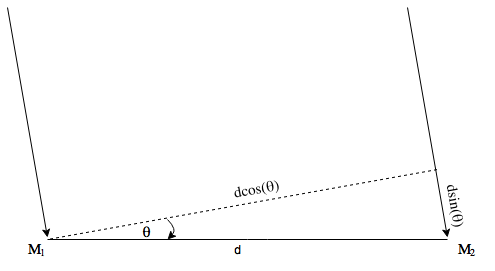
\includegraphics[width=0.8\textwidth]{Figures/AngularRes.png}
     \caption{Figure represents plane wave incidence on a microphone pair. For broadside incidence the time delay is the minimum = 0 between the two microphones. The next time delay allowed is $1/$fs, corresponding to travel distance of $c/$fs (c being the speed of sound). So we have  dsin($\theta$) = $c$/fs. For endside incidence the time delay is maximum = $d/c$. The next time delay allowed is $d/c$-$1/$fs, corresponding to travel distance of $d$-$c/$fs, and we have dsin($\theta$) =  $d$-$c/$fs.}
     \label{fig:ang_res}
\end{figure}

The issue is solved by curve fitting and interpolation. Parabolic curve fitting was initially proposed method to solve it, but was shown to be a biased estimator \cite{boucher1981analysis}. Consequently, various interpolation techniques have been developed to overcome this issue \cite{jacovitti1993discrete}, \cite{brandstein1997practical}, \cite{zhang2005cross}, \cite{tervo2008interpolation}. The 2D localization resolution with no interpolation is plotted in Fig. \ref{fig:res_diff}.

\begin{figure}[H]
    \centering
    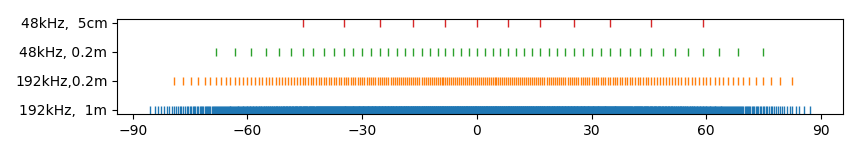
\includegraphics[width=\textwidth]{Figures/res_diff.png}
    \caption{Frontal 2D localization resolution for different sample rates and distance between a pair of microphones. As can be seen large apertures and high sample rates have a better resolution than lower sample rates and smaller apertures.}
    \label{fig:res_diff}
\end{figure}

Some simulations for GCC are given in Fig. \ref{fig:GCC_SIM}. It can be seen that the resolution falls the closer we get to end-side ($0\degree$ and $180\degree$). Also it can be seen that the results are poor if no weights are used. PHAT and SCOT perform quite similarly in the simulations, with PHAT being marginally better. It can be seen that the level difference is maintained between the 2 sources in the results. However no peaks are visible if the SNR falls to 0 dB.

\begin{figure}[H]
    \centering
    \begin{subfigure}[b]{0.48\textwidth}
    \centering
    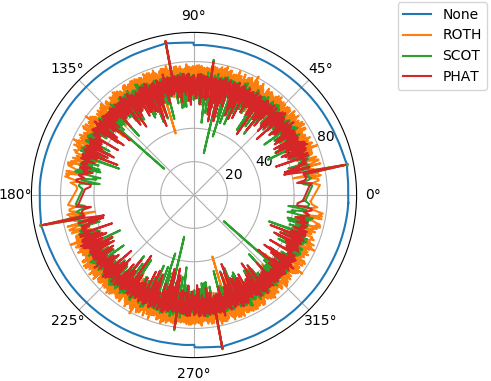
\includegraphics[width=0.9\textwidth]{Figures/GCC_40.png}
    \caption{Both sources at 40dB SNR}
    \label{fig:d1}
\end{subfigure}
\hfill
\begin{subfigure}[b]{0.48\textwidth}
    \centering
    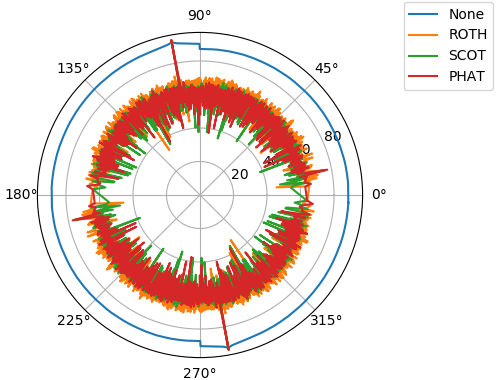
\includegraphics[width=0.9\textwidth]{Figures/GCC_20_40.png}
    \caption{S1 at 20dB SNR, S2 at 40dB SNR}
    \label{fig:d2}
\end{subfigure}
\vskip \baselineskip
\begin{subfigure}[b]{0.48\textwidth}
    \centering
    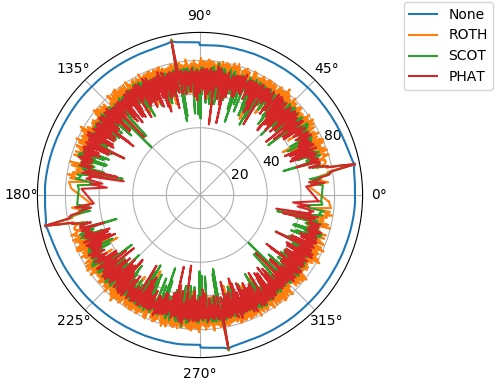
\includegraphics[width=0.9\textwidth]{Figures/GCC_20_20.png}
    \caption{Both sources at 20dB SNR}
    \label{fig:d3}
\end{subfigure}
\quad
\begin{subfigure}[b]{0.48\textwidth}
    \centering
    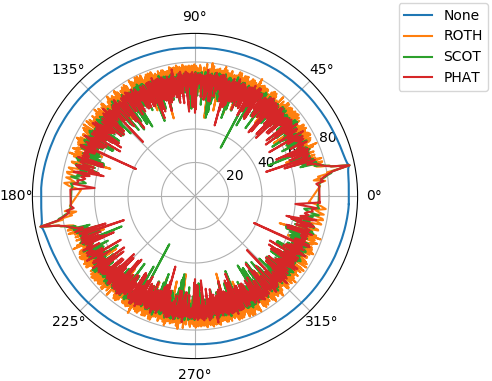
\includegraphics[width=0.9\textwidth]{Figures/GCC_0_20.png}
    \caption{S1 at 20 SNR, S2 at 0 SNR}
    \label{fig:d4}
\end{subfigure}
\caption{Figures compares different GCC algorithms for localization performance for 2 sources with various SNRs. The simulations assume 2 microphones placed 1m apart along the $0\degree-180\degree$ axis. The sampling rate is assumed to be 192kHz and speed of sound is 343m/sec. Two sources playing pink noise at different levels and located at $S_1:15\degree$ and $S_2:100\degree$ are assumed. Uncorrelated white noise is assumed to be present at the 2 microphones. No interpolation fixing is done. The level of the noise is unchanged but the level of the signal is varied to achieve the different SNRs.}
\label{fig:GCC_SIM}
\end{figure}


\subsection{Multiple pair GCC}

GCC equations described above are for a single pair of microphones only. Various algorithms have been designed that extend the GCC algorithm to multiple pairs of microphones. SRP-PHAT approach \cite{dibiase2000high} combines the steered response power (SRP) beamformer methods \cite{krim1996two} to the GCC approach. Griebel \cite{griebel2001microphone} describes a method where the \enquote{GCC functions derived from various microphone pairs are simultaneously maximized over a set of potential delay combinations consistent with candidate locations} which can be seen as a special case of SRP-PHAT where the redundant information from additional microphone pairs are utilized. \textit{Okuyama et al.} show in a 2002 study\cite{okuyama2002study} that when using a spatial array like a tetrahedron, the propagation direction of sound through the array can be determined, irrespective of the speed of sound, by using the least-squares approach. This means that for localizing sound sources outdoors, the instantaneous temperature and wind on the microphone array need not be known. Benesty \cite{benesty2004time} provides a method to fully utilize the redundant information from multiple microphone pairs to make the time-delay estimation (TDE) process more robust against distortion and also improve angular resolution. The method re-derives multi-channel cross correlation (MCCC) to apply linear interpolation on the GCC data to improve the angular resolution of localization. More recently, in \cite{liu2010continuous} the author used a motorized robot with 4 microphone arranged in a cross-formation. The algorithm uses 'de-noising' techniques such as adding a small regularization term to the denominator of the PHAT weight, which can reduce the low SNR issues surrounding PHAT. The low SNR regions can be further penalized by using reliability-weighted RW-PHAT \cite{valin2006robust}, where a-priori SNR information is used to estimate the weight to be multiplied during the PHAT computation. Eigenvalue decomposition based GCC (ES-GCC) is done by authors in \cite{hu2009estimation}. They conclude that ES-GCC produces less number of outlier locations that GCC-PHAT. Badali \cite{badali2009evaluating} compares various localization algorithms using a 8 microphone array located on a cube. The authors use hyperbolic intersection on the GCC results from multiple pairs of microphones. They conclude that if \textit{Direction Refinement} procedure is run, in which first a far-field assumption search is done and the locations are then 'refined' for near field, then the results from SRP-PHAT can be improved. But this procedure might not be relevant for far-field outdoor localization.  

The next sections will discuss some of the algorithms that are relevant for outdoor source localization and make the PHAT process more robust. 